\documentclass{swp1}
\usepackage[utf8]{inputenc}
\usepackage{amssymb}
\usepackage{url}


% Tabellen
\usepackage{tabularx}
\usepackage{supertabular}
\usepackage{booktabs}







\begin{document}

% \maketitle{Nummer}{Abgabedatum}{Tutor-Name}{Gruppennummer}
%           {Teilnehmer 1}{Teilnehmer 2}{Teilnehmer 3}
\maketitle{4}{13.07.2014}{Michaela Bunke}{ChronoX}
          {Tim Ellhoff}{Karsten Betjemann}{}
          
\section*{Aufgabe 1)}

\begin{figure}[h]
\centering{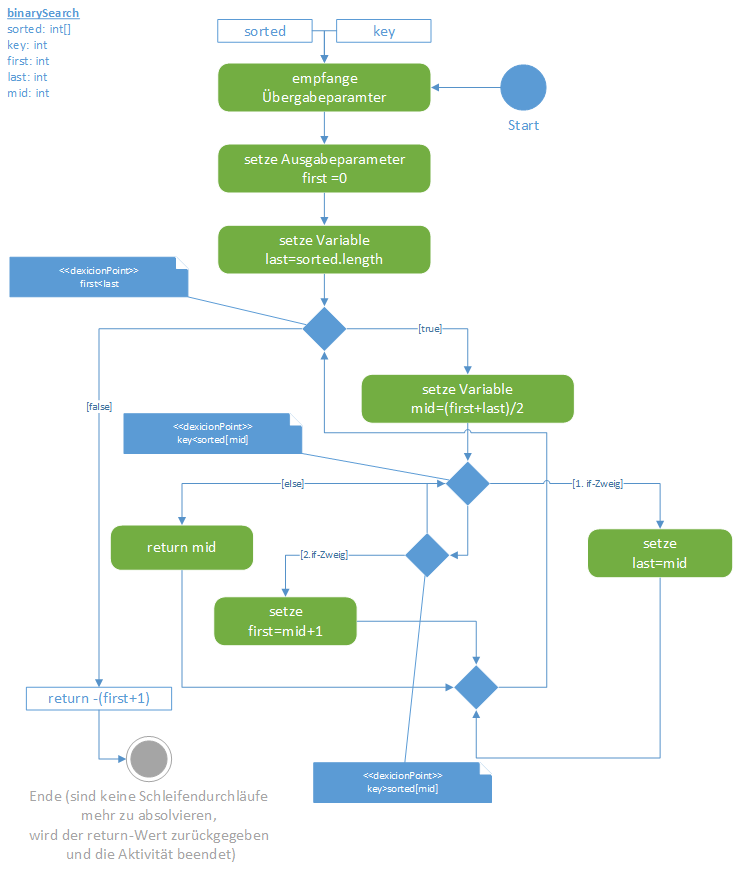
\includegraphics[width=13cm]{aufg1.png}}
\caption{Kontrollfluss der Java-Methode \texttt{binarySearch} in einem Aktivitätsdiagramm dargestellt}
\label{ab1}
\end{figure}


\section*{Aufgabe 2)}

\textbf{a.}\newline
\newline
In diesem Aktivitätsdiagramm wird - von der Bestellung bis zum Servieren - der Zubereitungsvorgang eines Kaffeeautomaten veranschaulicht.\newline
\newline
Der Ablauf des eigentlichen Prozesses gestaltet sich derart, als dass eine Bestellung beim Automaten eingeht \emph{(Take order)} und vonseiten des Automaten darauf geprüft wird, ob Tee oder Milchkaffee bestellt wurde.\newline
Bei einer Teebestellung gestaltet sich der Restverlauf des Diagramms simpel, die Zubereitung wird anschließend unter einem Punkt zusammgefasst \emph{(Make Tea)} und zuletzt wird dann das bestellte Getränk am Schlusspunkt des Aktivitätsdiagrammes serviert \emph{(Serve Drink)}.\newline
Beim Milchkaffee gestaltet sich der Prozess nur dahingehend komplizierter, als das die Zubereitung zunächst in die Herstellung des Kaffees \emph{(Make Coffee)} und das Aufschäumen der Milch \emph{(Steam Milk)} aufgeteilt wird, bevor diese Aktion im Hinzufügen der Milch zum Kaffee zusammenlaufen \emph{(Add Milk to Coffee)} und zuletzt auch zum Servieren als Schlusspunkt führen.\newline
\newline
Das Diagramm selbst weist im Bezug auf gängige Normen für Aktivitätsdiagramme Mängel auf, so wird beispielsweise die Grundregel von einem Aktionszustand mit nur einer Eingangsaktion dadurch verletzt, dass bei der Aufteilung der Nebenprozesse der Milchkaffeeherstellung der verwendete Fork Knoten nicht wieder zusammengeführt wird, was für sich bereits fehlerhaft ist und zu zwei Eingangsaktionen beim Hinzufügen der Milch zum Kaffee führt.
Diese Regel wird auch beim letzten Aktionszustand wieder verletzt, da die eigentliche Diagrammaufteilung in zwei Pfade durch jenen Bedingungsknoten, welcher die Art Bestellung prüft, hier nicht durch einen Merge-Knoten wieder zusammengeführt wurde.\newline
Dem gängigen Formalismus folgend ist es weiterhin ein Fehler, dass im Diagramm weder Startknoten noch Endknoten vorhanden sind. Das Diagramm beginnt und endet jeweils mit einem Aktionszustand.


\clearpage

\textbf{b.}\newline
\newline
\begin{figure}[h]
\centering{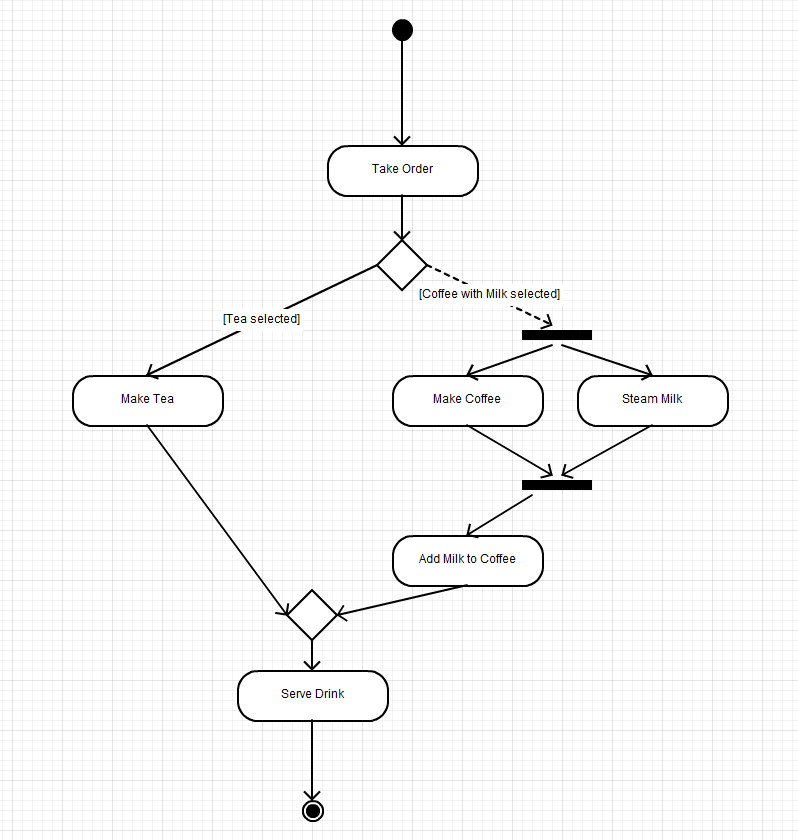
\includegraphics[width=13cm]{correct_diagramm.png}}
\caption{Korrigiertes Aktivitätsdiagramm}
\label{ab2}
\end{figure}
\newline
\clearpage

\section*{Aufgabe 3)}

\textbf{a.}\newline
\newline
\begin{figure}[h]
\centering{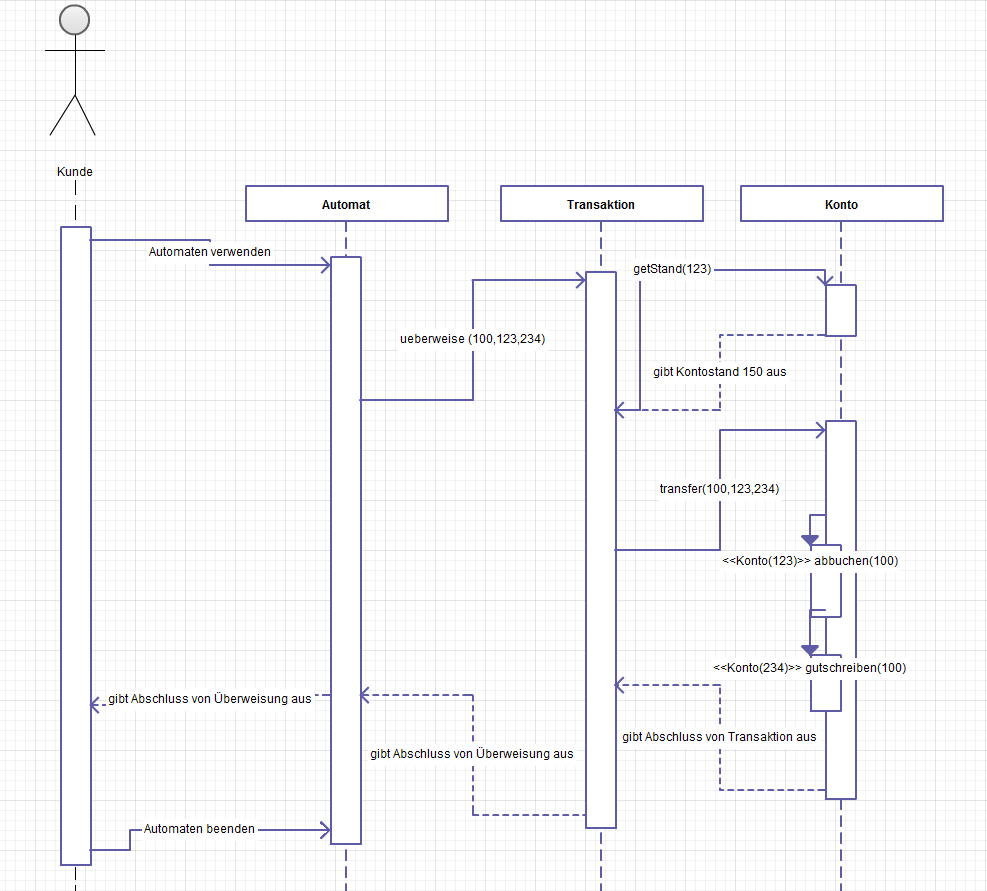
\includegraphics[width=13cm]{Automat a.png}}
\caption{Sequenzdiagramm 1 mit gedecktem Konto}
\label{ab3}
\end{figure}
\newline

\newpage

\textbf{b.}\newline
\newline
\begin{figure}[h]
\centering{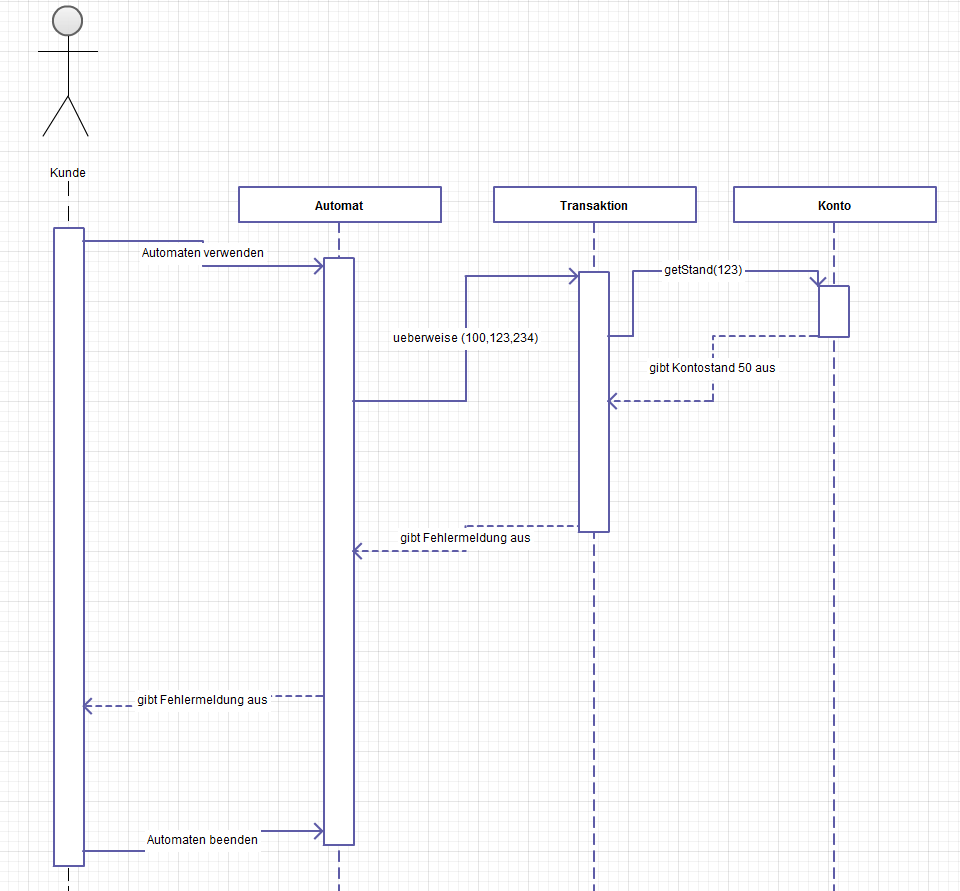
\includegraphics[width=13cm]{Automat b.png}}
\caption{Sequenzdiagramm 2 mit ungedecktem Konto}
\end{figure}
\newline
\section*{Aufgabe 4)}

Dargestellt ist der Ablauf in einem Online-Shop, visualisiert in einem Sequenzdiagramm. Dabei regelt die Klasse \texttt{ShoppingSession} die Shop-Sitzung und ist ebenso für die Darstellung des Shops zuständig. Die Klasse \texttt{Cart} stellt einen Einkaufswagen dar und die Klasse \texttt{ProductDB} repräsentiert den Zugriff auf die Produktdatenbank.

\textbf{Beschreibung des abgebildeten Vorgangs:}\\
Der Kunde ruft zunächst durch entsprechende Eingaben den Online-Shop auf. Es wird dabei eine Shop-Sitzung durch die Klasse \texttt{ShoppingSession} erstellt. Der Kunde sucht ein Notebook. Dazu gibt er in einem Suchfeld das Stichwort \glqq Notebook\grqq ein. Die \texttt{ShoppingSession} verarbeitet die Suchanfrage des Kunden und überprüft mit ihrer Methode \texttt{searchProducts} die Produktdatenbank \texttt{ProductDB} auf Treffer.\\
Die \texttt{ProductDB} liefert der \texttt{ShoppingSession} eine Liste mit Produkten zurück, die dem Kunden dann, wahrscheinlich in ansprechender Form (für die Darstellung ist auch die Klasse \texttt{ShoppingSession} zuständig) umgehend angezeigt wird.\\
der Kunde möchte sich Produktdetails von \textit{X123} anzeigen lassen. Die \texttt{ShoppingSession} ruft ihre Methode \texttt{getProductDetails} mit dem entsprechendem Parameter auf und fragt die Datenbank danach ab. \\
Die Datenbank liefert wiederum eine Liste mit Details zurück, die wieder in ansprechender Form dem Kunden von der \texttt{ShoppingSession} angezeigt werden.\\
Der Kunde entschließt sich dazu, das Gerät \texttt{X123} zu kaufen und legt es durch entsprechende Eingaben in den Warenkorb. Letzterer wird durch die Klasse \texttt{Cart} modelliert. Der Konstruktur der Klasse wird aufgerufen und mittels der \texttt{add}-Methode und dem entsprechendem Parameter wird das Gerät tatsächlich in den virtuellen Warenkorb bewegt, da die Methode \texttt{true} zurückliefert. Dies wird an die \texttt{ShoppingSession} weitergeleitet, die dann diese Information in verständlicher Form an den Kunden weiterleitet. \\
Zum Schluss überlegt es sich der Kunde doch noch mal anders und bricht seinen Einkauf ab, indem er durch entsprechende Eingaben (z.B. Löschen des Warenkorbs oder Ausloggen) der \texttt{ShoppingSession} den Abbruch mitteilt. Diese ruft die \texttt{clearProducts}-Methode auf und der entsprechende Teil der Datenbank wird geleert bzw. gelöscht. Schließlich liefert die Methode \texttt{true} zurück und die Aktion wurde erfolgreich abgebrochen. Der Warenkorb dürfte somit wieder leer sein.
\clearpage


\textbf{Äquivalentes Kommunikationsdiagramm:}
\begin{figure}[h]
\centering{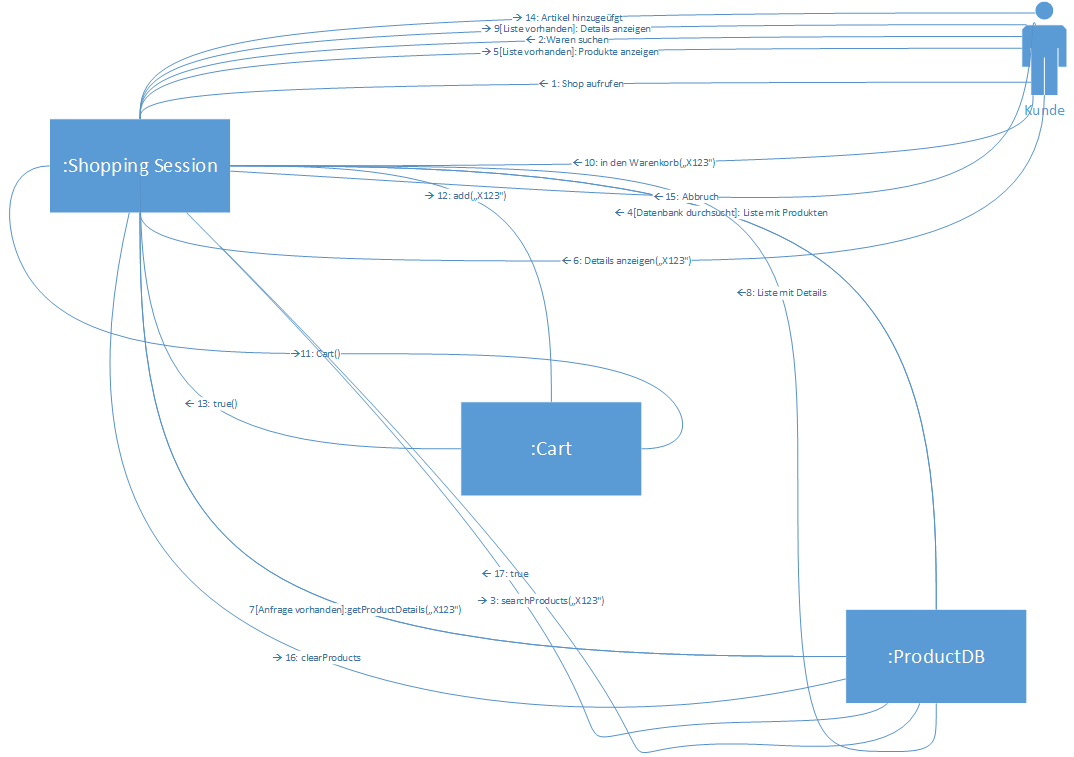
\includegraphics[width=16.5cm]{aufg4.png}}
\caption{Äquivalentes Kommunikationsdiagramm zum gegebenen Sequenzdiagramm}
\label{ab3}
\end{figure}

\end{document}

